%%%%%%%%%%%%%%%%%%%%%%%%%%%%%%%%%%%%%%%%%
% University Assignment Title Page 
% LaTeX Template
% Version 1.0 (27/12/12)
%
% This template has been downloaded from:
% http://www.LaTeXTemplates.com
%
% Original author:
% WikiBooks (http://en.wikibooks.org/wiki/LaTeX/Title_Creation)
%
% License:
% CC BY-NC-SA 3.0 (http://creativecommons.org/licenses/by-nc-sa/3.0/)
% 
% Instructions for using this template:
% This title page is capable of being compiled as is. This is not useful for 
% including it in another document. To do this, you have two options: 
%
% 1) Copy/paste everything between \begin{document} and \end{document} 
% starting at \begin{titlepage} and paste this into another LaTeX file where you 
% want your title page.
% OR
% 2) Remove everything outside the \begin{titlepage} and \end{titlepage} and 
% move this file to the same directory as the LaTeX file you wish to add it to. 
% Then add \input{./title_page_1.tex} to your LaTeX file where you want your
% title page.
%
%%%%%%%%%%%%%%%%%%%%%%%%%%%%%%%%%%%%%%%%%

%----------------------------------------------------------------------------------------
% PACKAGES AND OTHER DOCUMENT CONFIGURATIONS
%----------------------------------------------------------------------------------------

\documentclass[12pt]{article}
\usepackage{parskip}
\usepackage{enumitem}
\usepackage{setspace}
\usepackage{graphicx}
\usepackage[margin=1.0in] {geometry}
\usepackage[none] {hyphenat}
\setlength{\parindent}{10ex}
\newcommand*{\SignatureAndDate}[1]{%
    \par\noindent\makebox[2.5in]{\hrulefill} \hfill\makebox[2.0in]{\hrulefill}%
    \par\noindent\makebox[2.5in][l]{#1}      \hfill\makebox[2.0in][l]{Date}%
}%

\begin{document}
\begin{titlepage}

\newcommand{\HRule}{\rule{\linewidth}{0.5mm}} % Defines a new command for the horizontal lines, change thickness here

\center % Center everything on the page
 
%----------------------------------------------------------------------------------------
% HEADING SECTIONS
%----------------------------------------------------------------------------------------

\textsc{\LARGE University Of Tennessee\\ Knoxville}\\[1.5cm] % Name of your university/college
\textsc{\Large Art Of Hiking Application}\\[0.5cm] % Major heading such as course name
%\textsc{\large Team \#13}\\[0.5cm] % Minor heading such as course title

%----------------------------------------------------------------------------------------
% TITLE SECTION
%----------------------------------------------------------------------------------------

\HRule \\[0.4cm]
{ \huge \bfseries Description of Tables}\\[0.4cm] % Title of your document
\HRule \\[1.5cm]
 
%----------------------------------------------------------------------------------------
% AUTHOR SECTION
%----------------------------------------------------------------------------------------

\begin{minipage}{0.4\textwidth}
\begin{flushleft} \large
\emph{Authors:}\\
Gabriel \textsc{Hanas}\\
Chris \textsc{Tester}\\
Robert \textsc{Moncrief}\\
Trevor \textsc{Jones}\\
Anthony \textsc{Stewart}\\
\end{flushleft}
\end{minipage}
~
\begin{minipage}{0.4\textwidth}
\begin{flushright} \large
\emph{Customer:} \\
Bradley \textsc{Vander Zanden} % Supervisor's Name
\end{flushright}
\end{minipage}\\[4cm]

% If you don't want a supervisor, uncomment the two lines below and remove the section above
%\Large \emph{Author:}\\
%John \textsc{Smith}\\[3cm] % Your name

%----------------------------------------------------------------------------------------
% DATE SECTION
%----------------------------------------------------------------------------------------

{\large \today}\\[3cm] % Date, change the \today to a set date if you want to be precise

%----------------------------------------------------------------------------------------
% LOGO SECTION
%----------------------------------------------------------------------------------------

%\includegraphics{Logo}\\[1cm] % Include a department/university logo - this will require the graphicx package
 
%----------------------------------------------------------------------------------------

\vfill % Fill the rest of the page with whitespace

\end{titlepage}
\tableofcontents


\newpage
\section{Table: Region}
\subsection{Attributes}
\textbf{\underline{regionId:}}\\\\
\textbf{Can it be Null:} No\\
\textbf{Type:} Int\\
\textbf{Description:} An integer that will distinguish the region. Auto incremented.\\\\


\textbf{\underline{regionName:}}\\\\
\textbf{Can it be Null:} No\\
\textbf{Type:} Varchar (255)\\
\textbf{Description:} The name of the region.


\subsection{Keys}
\textbf{Primary Key} - \texttt{regionId}\\
The region table will use a standard incrementing regionID to 
list all of the warnings input by the users.
\subsection{Constraints:} Region names must be unique.



\newpage
\section{Table: Trail}
\subsection{Attributes}
\textbf{\underline{traiId:}}\\\\
\textbf{Can it be Null:} No\\
\textbf{Type:} Int\\
\textbf{Description:} A unique integer that identifies a trail. Auto incremented.\\\\


\textbf{\underline{trailName:}}\\\\
\textbf{Can it be Null:} No\\
\textbf{Type:} Varchar (255)\\
\textbf{Description:} A character string that corresponds to the trail name.\\\\


\textbf{\underline{trailLength:}}\\\\
\textbf{Can it be Null:} No\\
\textbf{Type:} Double (3,1)\\
\textbf{Description:} A doubleing point number representing the length
of a trail to one decimal point. \\\\


\textbf{\underline{trailDifficulty:}}\\\\
\textbf{Can it be Null:} Yes\\
\textbf{Type:} Double (3,2)\\
\textbf{Description:} A doubleing point number that represents the standard 
difficulty of a trail.\\\\


\textbf{\underline{elevationGain:}} \\\\
\textbf{Can it be Null:} No\\
\textbf{Type:} Double (6,2)\\
\textbf{Description:} An integer that represents the overall elevation gain of a trail. \\\\


\textbf{\underline{elevationGainMap:}}\\\\
\textbf{Can it be Null:} Yes\\
\textbf{Type:} Varchar (255)\\
\textbf{Description:} Unknown\\\\


\textbf{\underline{region:}}\\\\
\textbf{Can it be Null:} No\\
\textbf{Type:} Int \\
\textbf{Description:} An integer that defines which region a trail lies in. \\\\


\textbf{\underline{horseAccessible:}}\\\\
\textbf{Can it be Null:} No\\
\textbf{Type:} Boolean\\
\textbf{Description:} A true or false statement to indicate if horses are allowed 
on a trail. \\\\


\textbf{\underline{trailDescription:}}\\\\
\textbf{Can it be Null:} Yes\\
\textbf{Type:} Text\\
\textbf{Description:} A character string describing
the trail and its highlights. \\\\


\textbf{\underline{isLoop:}}\\\\
\textbf{Can it be Null:} No\\
\textbf{Type:} Boolean\\
\textbf{Description:} Tells if a trail is point to point or a loop.\\\\



\subsection{Keys}
\textbf{Primary Key} - \texttt{trailId}\\
\textbf{Foreign Key} - \texttt{region} (Links to Region table)\\
The \texttt{trailId} is the primary key because more than one trail can have the 
same name. The artificial key, \texttt{trailId} uniquely defines a trail.

\subsection{Constraints}
When inserting, the region must already exist. No two trails can have the same name in
the same region.
% END OF TRAIL TABLE 




\newpage
\section{Table: Intersection}
\subsection{Attributes}
\textbf{\underline{intersectionId:}}\\
%%
\\
\textbf{Can it be Null:} No \\
\textbf{Type:} Int\\
\textbf{Description:} A unique integer that identifies when two or more
trails intersect. Auto increment.\\\\
%%
\textbf{\underline{longitudePt:}}\\
%%
\\
\textbf{Can it be Null:} No\\
\textbf{Type:} Double\\
\textbf{Description:} A doubleing point number representing the 
longitudinal position of the intersection.\\\\
%%
\textbf{\underline{latitudePt:}}\\
%%
\\
\textbf{Can it be Null:} No\\
\textbf{Type:} Double\\
\textbf{Description:} A doubleing point number representing the 
latitudinal position of the intersection.\\\\
%%
\subsection{Keys}
\textbf{Primary Key} - \texttt{intersectionId}\\
The \texttt{intersectionId} is the primary key since it will uniquely define the intersection 
point. The other fields will give partial information to the location of the 
intersection but do not specify which intersection it is. 

\subsection{Constraints}
No special constraints.
%%End of Intersection Table

\newpage
\section{Table: InterestPointType}
\subsection{Attributes}
\textbf{\underline{typeId:}}\\
%%
\\
\textbf{Can it be Null:} No\\
\textbf{Type:} Int\\
\textbf{Description:}
An integer that uniquely identifies a point of interest. Auto increment.\\\\
%%
\textbf{\underline{interestPointDescription:}}\\
%%
\\
\textbf{Can it be Null:} Yes\\
\textbf{Type:} Varchar\\
\textbf{Description:} A short description 
of the interest point type. \\\\


\subsection{Keys}
\textbf{Primary Key} - \texttt{typeId}\\
The \texttt{typeId} is the primary key, because if a point of interest 
exists, it will always have an id number. There is no 
guarantee there will be a description available for that interest point.
\subsection{Constraints} 
As long as the entry exists there are not any constraints 
on the data since it is only a description.
%%
%End of IPT table 

\newpage
\section{Table: InterestPoint}
\subsection{Attributes}
\textbf{\underline{interestPointId:}}\\
%%
\\
\textbf{Can it be Null:} No\\
\textbf{Type:} Int\\
\textbf{Description:} A unique integer that identifies an interest point. Auto increment.\\\\
%%
\textbf{\underline{interestPointName:}}\\
%%
\\
\textbf{Can it be Null:} Yes\\
\textbf{Type:} Varchar\\
\textbf{Description:} The name of an interest point, if applicable. \\\\
%%
\textbf{\underline{typeId:}}\\
%%
\\
\textbf{Can it be Null:} No\\
\textbf{Type:} Int\\
\textbf{Description:} An integer that defines what type of interest point the data is. \\\\
%%
\textbf{\underline{latitudePoint:}}\\
%%
\\
\textbf{Can it be Null:} No\\
\textbf{Type:} Double\\
\textbf{Description:}
The latitudinal location of a trail point. \\\\
%%
\textbf{\underline{longitudePoint:}}\\
%%
\\
\textbf{Can it be Null:} No\\
\textbf{Type:} Double\\
\textbf{Description:}
The longitudinal location of a trail point.\\\\
%%
\subsection{Keys}
\textbf{Primary Key} - \texttt{interestPointId}\\
\textbf{Foreign Key} - \texttt{typeId} (Links to Interest Point)\\
The \texttt{interestPointId} is the primary key since it is the only field
that uniquely identifies the point of interest. For 
\texttt{interestPointName}, as the application expands there is a possibility of two points of interest with the same name to exist. 

\subsection{Constraints}
When an interest point is created, it must have a type.
%%
%End of Table



\newpage
\section{Table: ParkingLot}
\subsection{Attributes}
\textbf{\underline{parkingLotId:}}\\
%%
\\
\textbf{Can it be Null:} No\\
\textbf{Type:} Int\\
\textbf{Description:}
An integer specific to the parking lot. Auto increment.\\\\
%%
\textbf{\underline{maxLotCapacity:}}\\
%%
\\
\textbf{Can it be Null:} Yes\\
\textbf{Type:} Int\\
\textbf{Description:}
An integer number that represents the maximum amount of parking spots the given lot has.\\\\
%%
\textbf{\underline{latitudePoint:}}\\
%%
\\
\textbf{Can it be Null:} No\\
\textbf{Type:} Double\\
\textbf{Description:}
The latitudinal location of the parking lot. \\\\
%%
\textbf{\underline{longitudePoint:}}\\
%%
\\
\textbf{Can it be Null:} No\\
\textbf{Type:} Double\\
\textbf{Description:}
The longitudinal location of the parking lot.\\\\
%%
\subsection{Keys}
\textbf{Primary Key} - \texttt{parkingLotId}\\
The \texttt{parkingLotId} is the primary key because no other feilds can describe it.
\subsection{Constraints}
No special constraints.
%End Of parking lot table 



\newpage
\section{Table: TrailPoint}
\subsection{Attributes}
\textbf{\underline{trailPointId:}}\\
%%
\\
\textbf{Can it be Null:} No\\
\textbf{Type:} Int\\
\textbf{Description:}
The Id for a point along a specific trail. Auto increment.\\\\
%%
\textbf{\underline{latitudePoint:}}\\
%%
\\
\textbf{Can it be Null:} No\\
\textbf{Type:} Double\\
\textbf{Description:}
The latitudinal location of a trail point. \\\\
%%
\textbf{\underline{longitudePoint:}}\\
%%
\\
\textbf{Can it be Null:} No\\
\textbf{Type:} Double\\
\textbf{Description:}
The longitudinal location of a trail point.\\\\
%%
\textbf{\underline{elevationPoint:}}\\
%%
\\
\texbf{Can in be Null:} No\\
\textbf{Type:} Double\\
\textbf{Description:}
The elevation location of a trail point.\\\\
%%
\textbf{\underline{trailId:}}\\%% what is this used for?
%%
\\
\textbf{Can it be Null:} No\\
\textbf{Type:} Int\\
\textbf{Description:}
An integer that corresponds to a trail. This is okay because we will 
duplicate trailPoints that lie on multipe trails.\\\\
%%
\textbf{\underline{previousPoint:}}\\
%%
\\
\textbf{Can it be Null:} Yes\\
\textbf{Type:} Int\\
\textbf{Description:}
An integer that corresponds to the next trail point. If null, it is the 'common' start of a trail.\\\\
%%
\subsection{Keys}
\textbf{Primary Key} - \texttt{trailPointId}\\
\textbf{Foreign Key} - \texttt{trailId} (Links to Trail)\\
\textbf{Foreign Key} - \texttt{previousPoint} (Links to TrailPoint)\\
The trail point table will hold a list of points that make up 
a given trail. They will be marked by longitudinal and latitudinal
points from the map. Each point will be given a unique id. If trails
share a point, the point will be duplicated in these cases.

\subsection{Constraints:}
No unique constraints.
%% End of trail points table



\newpage
\section{Table: TrailHead}
\subsection{Attributes}
\textbf{\underline{trailHeadId:}}\\
%%
\\
\textbf{Can it be Null:} No\\
\textbf{Type:} Int\\
\textbf{Description:}
An integer that will distinguish all the beginnings of trails. Auto increment.\\\\
%%
\textbf{\underline{parkingLotId:}}\\
%%
\\
\textbf{Can it be Null:} Yes\\
\textbf{Type:} Int\\
\textbf{Description:}
A unique integer that will match the starting point to a 
parking lot if available. \\\\
%%
\textbf{\underline{trailPoint:}}\\ %% what is this?
%%
\\
\textbf{Can it be Null:} No\\
\textbf{Type:} Int\\
\textbf{Description:}
The id for a starting trail point.\\\\
%%

\subsection{Keys}
\textbf{Primary Key} - \texttt{trailHeadId}\\
\textbf{Foreign Key} - \texttt{parkingLotId} (Links to ParkingLot)\\
\textbf{Foreign Key} - \texttt{trailPt} (Links to Trail)\\
The trail head table will contain the starting points of trails
and any parking lot that is connected to them. The \texttt{trailHeadId} will be 
unique to allow the user to select either end if the trail is has
more than on starting position. 

\subsection{Constraints:}
The only constraint is the head point must be connected to a trail 
that already exists in the database.



\newpage
\section{Table: Warnings}
\subsection{Attributes}
\textbf{\underline{warningId:}}\\
%%
\\
\textbf{Can it be Null:} No\\
\textbf{Type:} Int\\
\textbf{Description:}
An integer that will distinguish the Warning.\\\\
%%
\textbf{\underline{trailId:}}\\
%%
\\
\textbf{Can it be Null:} Yes\\
\textbf{Type:} Int\\
\textbf{Description:}
A unique integer that will match the warning to a specific trail. \\\\
%%
\textbf{\underline{regionId:}}\\ %
%%
\\
\textbf{Can it be Null:} Yes\\
\textbf{Type:} Int\\
\textbf{Description:}
A unique integer that will match the warning to a specific region. \\\\
%%
\textbf{\underline{dateEntered:}}\\ 
%%
\\
\textbf{Can it be Null:} No\\
\textbf{Type:} DateTime\\
\textbf{Description:}
The date that the warning was entered.\\\\
%%

\textbf{\underline{warningText:}}\\
%%
\\
\textbf{Can it be Null:} Yes\\
\textbf{Type:} Text\\ %Fix it laters
\textbf{Description:}
The text of the warning. \\\\
%%


\subsection{Keys}
\textbf{Primary Key} - \texttt{warningId}\\
\textbf{Foreign Key} - \texttt{trailId}\\
\textbf{Foreign Key} - \texttt{regionId}\\
The warning table will use a standard incrementing warningID to 
list all of the warnings input by the users.
\subsection{Constraints:}
Either the regionId or the trailId must be valid. 

\newpage



\newpage
\section{Table: User}
\subsection{Attributes}
\textbf{\underline{userId:}}\\
%%
\\
\textbf{Can it be Null:} No\\
\textbf{Type:} Int \\
\textbf{Description:} 
A unique integer that identifies a user to the database. Auto increment.\\\\
%%
\textbf{\underline{username:}}\\
%%
\\
\textbf{Can it be Null:} No \\
\textbf{Type:} Varchar\\
\textbf{Description:} A picked username that will be used to log in 
for writing reviews.\\\\
%%
\textbf{\underline{password:}}\\
%%
\\
\textbf{Can it be Null:} No\\
\textbf{Type:} Varchar\\
\textbf{Description:} A user designated password to sign into their account.\\\\
%%
\textbf{\underline{email:}}\\
%%
\\
\textbf{Can it be Null:} No\\
\textbf{Type:} Varchar\\
\textbf{Description:} A email to allow the user account to be validated. \\\\
%%
\subsection{Keys}
\textbf{Primary Key} - \texttt{userId}\\
The \texttt{userId} is the primary key to retain all artificial keys as 
primary keys throughout the database for consistency. \texttt{username} is a candidate key since it is unique.

\subsection{Constraints} 
Once the user is created, there will be constraints on the \texttt{password} and \texttt{username}.
The \texttt{password} will have to be at least eight characters and contain letters and numbers.
The \texttt{password} will also be salted and hashed for security.
The \texttt{username} has to be unique and be between 6 and 20 characters. 
%%End of User Table





\newpage
\section{Table: Review}
\subsection{Attributes}
\textbf{\underline{reviewId:}}\\
%%
\\
\textbf{Can it be Null:} No\\
\textbf{Type:} Int \\
\textbf{Description:} An integer that uniquely identifies the review. Auto increment.\\\\
%%
\textbf{\underline{userId:}}\\
%%
\\
\textbf{Can it be Null:} No\\
\textbf{Type:} Int\\
\textbf{Description:} An integer that links a review to its author.\\\\
%%
\textbf{\underline{trailId:}}\\
%%
\\
\textbf{Can it be Null:} No\\
\textbf{Type:} Int\\
\textbf{Description:} An integer that links a review to a specific trail.\\\\
%%
\textbf{\underline{userRating:}}\\
%%
\\
\textbf{Can it be Null:} Yes\\
\textbf{Type:} Int\\
\textbf{Description:} An integer, one through five, that relates to how 
much a user liked a trail. \\\\
%%
\textbf{\underline{userReview:}}\\
%%
\\
\textbf{Can it be Null:} Yes\\
\textbf{Type:} Text\\
\textbf{Description:} A written review that describes what a user 
liked or disliked about a trail.\\\\
%%
\subsection{Keys}
\textbf{Primary Key} - \texttt{reviewId}\\
\textbf{Foreign Key} - \texttt{userId} (Links to User table)\\
\textbf{Foreign Key} - \texttt{trailId} (Links to Trail table)\\
The \texttt{reviewId} is the primary key since the \texttt{userRating} and \texttt{userReview} are not unique fields.

\subsection{Constraints} 
A user must make a rating and/or a review.
Once a review or rating is created it must be linked to a user and trail.
%%End of Review Table




\newpage
\section{Table: TrailIntersectionMapping}
\subsection{Attributes}
\textbf{\underline{trailId:}}\\
%%
\\
\textbf{Can it be Null:} No \\
\textbf{Type:} Int \\
\textbf{Description:} A unique integer that corresponds with a trail. \\\\
%%
\textbf{\underline{intersectionId:}}\\
%%
\\
\textbf{Can it be Null:} No \\
\textbf{Type:} Int \\
\textbf{Description:} A unique integer that corresponds with an intersection. \\\\
%%

\subsection{Keys}
\textbf{Foreign Key} - \texttt{trailId} (Links to Trail table)\\
\textbf{Foreign Key} - \texttt{intersectionId} (Links to Intersection table)\\
The desired intersection is found by using the \texttt{trailId} and the \texttt{intersectionId} to create a 
\texttt{trailIntersectionId}.

\subsection{Constraints} 
When the table is entered there must be a \texttt{trailId} and an \texttt{intersectionId} in 
order to insert. 
%%End of Table












\newpage
\section{Table: InterestPointTrailMapping}
\subsection{Attributes}
\textbf{\underline{trailId:}}\\
%%
\\
\textbf{Can it be Null:} No\\
\textbf{Type:} Int\\
\textbf{Description:} An integer that represents a trail.

%%
\textbf{\underline{interestPointId:}}\\
%%
\\
\textbf{Can it be Null:} No\\
\textbf{Type:} Int\\
\textbf{Description:}  An integer representing an interest point.\\\\

\subsection{Keys}
\textbf{Foreign Key} - \texttt{trailId} (Links to Trail table)\\
\textbf{Foreign Key} - \texttt{interestPointId} (Links to InterestPoint table)\\
The junction table will use the two foreign keys together to find the specific
trail that a specific point of interest lies on, this junction table is needed when one point of interest is on multiple trails.

\subsection{Constraints}
When the table is entered there must be a \texttt{trailId} and an \texttt{interestPointId} in order to find the needed information.
%%
%End OF TABLE








\newpage
\section{Table: ParkingLotTrailMapping}
\subsection{Attributes}
\textbf{\underline{parkingLotId:}}\\
%%
\\
\textbf{Can it be Null:} No\\
\textbf{Type:} Int\\
\textbf{Description:}
An integer number that represents a parking lot. \\\\
%%
\textbf{\underline{trailId:}}\\
%%
\\
\textbf{Can it be Null:} No\\
\textbf{Type:} Int\\
\textbf{Description:}
An integer number that represents a trail.
%%

\subsection{Keys}
\textbf{Foreign Key} - \texttt{parkingLotId} (Links to ParkingLot table)\\
\textbf{Foreign Key} - \texttt{trailId} (Links to Trail)\\
The junction table will use the two foreign keys together to find the specific
parking lot that a specific trail is connected to. This junction table is useful when one parking lot connects to multiple trails
or a trail has multiple parking lots linked to it.

\subsection{Constraints:}
When the table is entered there must be a \texttt{parkingLotId} and an \texttt{trailId} in order to find the needed information.
%%
%End of junction Table 










\newpage
\section{ER Diagram}
\begin{center}
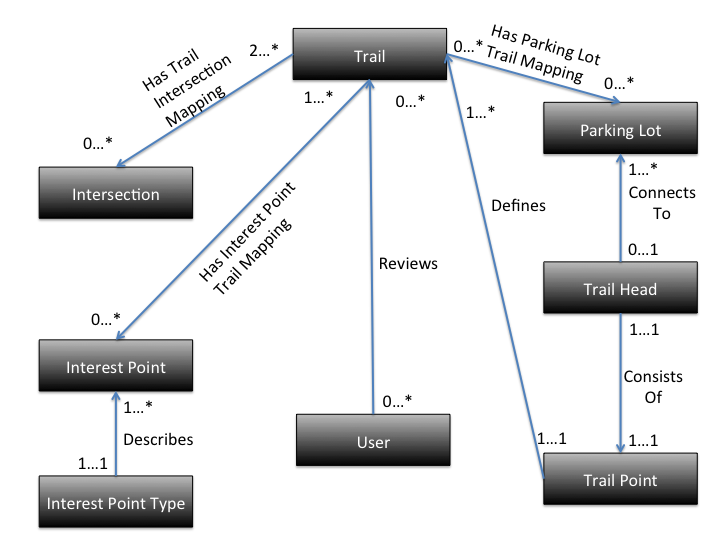
\includegraphics[scale=0.75]{ER_Diagram}
\end{center}

\end{document}
